\section{Canonical points from convex finite clouds}
\label{sec:convex-selector}

This section supplies a concrete extension of the existing finite-observation
library.  Its input may describe a convex set containing infinitely many points;
the construction nevertheless returns one canonical coherent point.  The
construction does not ask for a unique original witness.  Instead, it minimizes
squared distance to a specified anchor and derives a quantitative uniqueness
estimate directly from finite midpoint comparisons.

The distinction from the existing strong-minimizer adapter is precise.  At the
pinned repository revision, \texttt{Foundations/StrongMinimizer.lean} expresses
an objective numerator as \(I+R(y)\), where \(R\) is a natural-valued residual;
identifying this residual with the objective gap is an explicit application
obligation.  Here neither an exact optimum value nor a computable objective-gap
residual is an input.  Both selected objective values are compared with an
approximately available common midpoint, and the unknown optimum cancels.
The underlying geometry is classical; the contribution is the complete finite
interface, explicit schedule, and an adapter obligation that this interface
removes.  No historical priority claim is intended.

\subsection{The finite rational interface}

Fix integers \(d\geq 1\) and \(B\geq 1\).  A point is a vector in
\(\mathbb Q^d\).  Write
\[
 d_\infty(x,y)=\max_{i<d}|x_i-y_i|,
 \qquad Q(x,y)=\sum_{i<d}(x_i-y_i)^2,
 \qquad F_z(x)=Q(x,z).
\]
These are rational-valued primitive-recursive operations on finite codes.
In particular, no square-root operation is needed.  A cloud is a nonempty
finite list of points, with repetitions allowed.  Its representation includes
the list length and a bound \(|x_i|\leq B\) on every coordinate.
In dimension zero the unique empty vector is returned and every estimate is
zero.  A zero-sized geometric box can always use the harmless integer bound
\(B=1\).  Empty clouds are excluded because a nearest point to an empty set
is not defined.

For two clouds define their rational Hausdorff distance by
\[
 H_\infty(S,T)=\max\left\{
   \max_{x\in S}\min_{y\in T}d_\infty(x,y),
   \max_{y\in T}\min_{x\in S}d_\infty(x,y)\right\}.
\]
All maxima and minima are finite folds; a least index resolves a tie.  Define
the midpoint defect
\[
 M(S)=\max_{x,y\in S}\min_{w\in S}
       d_\infty\left(w,\frac{x+y}{2}\right).
\]
Thus \(M(S)\leq\eta\) is exactly the finite statement that every pair has a
cloud point within \(\eta\) of its midpoint.  This condition concerns the
cloud itself and is fully checkable by rational arithmetic.  One can instead
supply a primitive-recursive midpoint-index certificate, which is cheaper to
verify than computing the displayed maximum.

For an anchor \(z\in[-B,B]^d\cap\mathbb Q^d\), let
\(\operatorname{pick}(S,z)\) be the point at the least index minimizing
\(F_z\) on \(S\).  This is a bounded rational comparison loop.  An
\(\epsilon\)-minimizer means a point \(x\in S\) satisfying
\[
 F_z(x)\leq F_z(w)+\epsilon\qquad(w\in S),
 \quad \epsilon\geq 0.
\]
An exact finite minimizer is the case \(\epsilon=0\).

\begin{lemma}[The two finite identities]
\label{lem:cloud-identities}
For \(x,y,z\in[-B,B]^d\), put \(L=4dB\).  Then
\[
 |F_z(x)-F_z(y)|\leq Ld_\infty(x,y),
 \qquad
 F_z\left(\frac{x+y}{2}\right)
   =\frac{F_z(x)+F_z(y)}2-\frac{Q(x,y)}4.
\]
Also \(d_\infty(x,y)^2\leq Q(x,y)\).
\end{lemma}

\begin{proof}
For each coordinate,
\[
 (x_i-z_i)^2-(y_i-z_i)^2
 =(x_i-y_i)(x_i+y_i-2z_i),
 \qquad |x_i+y_i-2z_i|\leq4B.
\]
Sum these inequalities to obtain the first bound.  Expanding the two squares
in each coordinate gives the midpoint identity.  Each summand in \(Q\) is
nonnegative, so the largest coordinate square is at most their sum.
The proof uses only ordered rational arithmetic and induction on a finite
sum.  After clearing positive denominators, the induction invariant is
quantifier-free.
\end{proof}

\begin{theorem}[Finite comparison without an optimum value]
\label{thm:cloud-pair}
Let \(S,T\subset[-B,B]^d\) be nonempty finite rational clouds and
\(z\in[-B,B]^d\).  Suppose
\[
 H_\infty(S,T)\leq h,\qquad M(S)\leq\eta_S,
 \qquad M(T)\leq\eta_T.
\]
If \(x\) and \(y\) are, respectively, \(\epsilon_S\)- and
\(\epsilon_T\)-minimizers of \(F_z\), then
\begin{equation}
 \label{eq:cloud-pair}
 Q(x,y)\leq
  2L(\eta_S+\eta_T+h)+2(\epsilon_S+\epsilon_T),
 \qquad L=4dB.
\end{equation}
\end{theorem}

\begin{proof}
Choose a least-index point \(y'\in S\) with
\(d_\infty(y',y)\leq h\), and then a least-index point \(w_S\in S\)
with
\(d_\infty(w_S,(x+y')/2)\leq\eta_S\).  These are bounded choices
over the input lists.  If \(m=(x+y)/2\), the triangle inequality gives
\[
 d_\infty(w_S,m)\leq\eta_S+h/2.
\]
Every point here lies in the coordinate box, including \(m\).  Finite
near-minimality and Lemma~\ref{lem:cloud-identities} therefore give
\[
 F_z(x)\leq F_z(w_S)+\epsilon_S
 \leq F_z(m)+L(\eta_S+h/2)+\epsilon_S.
\]
Interchanging \(S,x\) and \(T,y\) gives
\[
 F_z(y)\leq F_z(m)+L(\eta_T+h/2)+\epsilon_T.
\]
Add the two inequalities and substitute
\(2F_z(m)=F_z(x)+F_z(y)-Q(x,y)/2\).
The objective values cancel, leaving \eqref{eq:cloud-pair}.
This cancellation is the reason that the exact minimum and its residual are
unnecessary.
\end{proof}

\begin{theorem}[Moving anchors]
\label{thm:cloud-moving-anchor}
Under the same cloud hypotheses, let \(x\) be an
\(\epsilon_S\)-minimizer of \(F_z\) on \(S\), and let \(y\) be an
\(\epsilon_T\)-minimizer of \(F_w\) on \(T\), where both anchors belong
to \([-B,B]^d\).  Then
\begin{equation}
 \label{eq:cloud-anchor}
 Q(x,y)\leq
 4L(\eta_S+\eta_T+h)+4Q(z,w)+4(\epsilon_S+\epsilon_T).
\end{equation}
\end{theorem}

\begin{proof}
The two midpoint comparisons now use different squared-distance objectives.
With \(A=L(\eta_S+\eta_T+h)+\epsilon_S+\epsilon_T\), their sum is
\[
 \frac{Q(x,y)}2
 \leq A+\sum_{i<d}(z_i-w_i)(x_i-y_i).
\]
This identity follows by expanding squares; the anchor-dependent difference
\(F_z-F_w\) is affine in the point.  Nonnegativity of
\(\sum_i((x_i-y_i)-2(z_i-w_i))^2\) gives
\[
 4\sum_i(z_i-w_i)(x_i-y_i)\leq Q(x,y)+4Q(z,w).
\]
Substitute this bound in the previous inequality and rearrange.
No division by a distance, and no case distinction concerning zero distance,
is used.
\end{proof}

\subsection{A coherent point from nonunique witnesses}

For \(n\in\mathbb N\), put \(r_n=2^{-n}\).  A convex cloud
presentation is a fixed primitive-recursive list program \(n\mapsto S_n\)
with proof contracts
\begin{align}
 &S_n\ne\varnothing,\qquad |(S_n[j])_i|\leq B,\label{eq:cloud-box}\\
 &H_\infty(S_n,S_m)\leq r_n+r_m,\label{eq:cloud-cauchy}\\
 &M(S_n)\leq2r_n.\label{eq:cloud-midpoint}
\end{align}
The phrase ``fixed primitive-recursive program'' matters: this is a schema
over specified programs, or a parameterized family with an explicit clock,
not a primitive-recursive evaluator for arbitrary program codes.

\begin{theorem}[Canonical finite-cloud selector]
\label{thm:convex-cloud-selector}
Let \((S_n)\) satisfy \eqref{eq:cloud-box}--\eqref{eq:cloud-midpoint},
and let \(z\in[-B,B]^d\cap\mathbb Q^d\).  Choose any integer \(c\)
such that \(2^c\geq24dB\), and define
\[
 N(k)=2k+c,\qquad
 q_k=\operatorname{pick}(S_{N(k)},z).
\]
Then \(k\mapsto q_k\) is primitive recursive and
\begin{equation}
 \label{eq:cloud-name}
 d_\infty(q_k,q_\ell)\leq2^{-k}+2^{-\ell}
 \qquad(k,\ell\in\mathbb N).
\end{equation}
The conclusion remains valid for independently selected finite minimizers;
ties and changing list order cannot change the represented point.
\end{theorem}

\begin{proof}
Apply Theorem~\ref{thm:cloud-pair} with \(\epsilon_S=\epsilon_T=0\).
The midpoint and Hausdorff bounds give
\[
 Q(\operatorname{pick}(S_n,z),\operatorname{pick}(S_m,z))
 \leq 24dB(r_n+r_m).
\]
Consequently
\[
 d_\infty(q_k,q_\ell)^2
 \leq 24dB\,2^{-c}(2^{-2k}+2^{-2\ell})
 \leq (2^{-k}+2^{-\ell})^2.
\]
Both sides being squares of nonnegative rationals, their rational order gives
\eqref{eq:cloud-name}.  A suitable \(c\) can be found by a bounded scan
through \(0,\ldots,24dB\), since \(2^{24dB}\geq24dB\).
Thus even selecting the schedule is primitive recursive.
\end{proof}

This is not an application of an infinite branch principle.  At query
precision \(k\), the algorithm makes just one cloud query and one finite
minimization.  The theorem proves directly that all such independently
computed answers fit together.

\begin{corollary}[An anchor supplied by a name]
\label{cor:cloud-anchor-name}
Suppose rational anchors \(z_n\in[-B,B]^d\) satisfy
\(d_\infty(z_n,z_m)\leq r_n+r_m\).
Set \(q_k=\operatorname{pick}(S_{2k+c},z_{2k+c})\), where
\(2^c\geq56dB\).  Then \eqref{eq:cloud-name} holds.
\end{corollary}

\begin{proof}
Let \(s=r_n+r_m\leq2\).  Theorem~\ref{thm:cloud-moving-anchor} gives
\[
 Q(\operatorname{pick}(S_n,z_n),\operatorname{pick}(S_m,z_m))
 \leq48dB\,s+4d s^2
 \leq56dB\,s,
\]
where \(s^2\leq2s\) and \(B\geq1\) were used.  Apply the same
dyadic schedule argument.
\end{proof}

\subsection{Meaning of the represented point}

The preceding theorems are finite arithmetic statements.  Their ordinary
mathematical meaning is recorded separately so that a semantic completion
argument is not misreported as a formalized iPRA proof.

Suppose a nonempty compact convex set \(K\subset[-B,B]^d\) is represented
by clouds with \(H_\infty(S_n,K)\leq r_n\).  The Hausdorff triangle
inequality implies \eqref{eq:cloud-cauchy}.  If \(u,v\in S_n\), choose
points \(a,b\in K\) within \(r_n\) of them.  Convexity puts
\((a+b)/2\) in \(K\), and some cloud point is within \(r_n\) of that
midpoint.  It is within \(2r_n\) of \((u+v)/2\), proving
\eqref{eq:cloud-midpoint}.  In a represented-space formulation the finite
cover witnesses supply these comparisons; no oracle deciding arbitrary
real equality is needed.

The name \((q_k)\) has an ordinary Euclidean limit \(q\).  Since its
distance from \(K\) tends to zero, \(q\in K\).  For each \(a\in K\),
there is a point \(a_k\in S_{N(k)}\) with
\(d_\infty(a_k,a)\leq r_{N(k)}\).  Finite minimality yields
\(F_z(q_k)\leq F_z(a_k)\); passing to the limit proves
\[
             F_z(q)\leq F_z(a)\qquad(a\in K).
\]
If \(q'\) has the same minimizing property, the exact midpoint identity
and convexity imply \(Q(q,q')=0\).  Therefore \(q\) is the unique
Euclidean metric projection of \(z\) on \(K\).

The same argument can be phrased entirely as observations of names.
For a membership witness at a prescribed precision, finite covering gives
a cloud competitor; finite minimization gives a rational objective
comparison with an explicit error; increasing the query precision removes
that error in the represented-order interface.  These are the concrete
object-theory obligations for the minimum-property endpoint.  They do not
require a term for the exact infimum.

More generally, the cloud contracts themselves suffice to define a semantic
closed set
\[
 K=\{a\in[-B,B]^d:
            \operatorname{dist}_\infty(a,S_n)\leq r_n\text{ for all }n\}.
\]
The constructed \(q\) belongs to it, because
\(\operatorname{dist}_\infty(q_m,S_n)\leq r_m+r_n\) before taking a
limit.  For \(a,b\in K\), approximate them at a very fine stage \(m\),
repair the midpoint there, and transfer to a fixed stage \(n\).  This gives
\[
 \operatorname{dist}_\infty((a+b)/2,S_n)\leq r_n+4r_m.
\]
Letting \(m\) increase proves midpoint closure of \(K\).  Its closedness
then gives closure under all real convex combinations by dyadic
approximation.  The finite estimate \(r_n+4r_m\), rather than an
unexplained compactness assertion, is the iPRA-facing content of this step.

\subsection{An explicit producer: convex hulls with degeneracies}

The input interface is substantive, so an explicit producer is useful.
Suppose \(v_1,\ldots,v_m\in[-B,B]^d\), where \(m\geq1\), are given
by one fixed primitive-recursive family \(V(p,j,t)\), with persistent data \(p\), internal vertex index \(j<m\), and precision \(t\). Write \(V_j(t)=V(p,j,t)\). Assume these names satisfy
\[
 d_\infty(V_j(t),V_j(s))\leq2^{-t}+2^{-s}.
\]
Clamp each coordinate of \(V_j(t)\) to \([-B,B]\).  Clamping is a
rational operation that is nonexpansive in the maximum norm, so it
preserves the displayed estimate and any interpretation in the box.
Use the clamped names below.

Set
\[
 t_n=n+1,\qquad D_n=4Bm\,2^n,
\]
and enumerate the cloud
\begin{equation}
 \label{eq:hull-cloud}
 S_n=\left\{\sum_{j=1}^m\frac{a_j}{D_n}V_j(t_n):
       a_j\in\{0,\ldots,D_n\},\quad\sum_{j=1}^ma_j=D_n\right\}.
\end{equation}
It is nonempty, for example by choosing \(a_1=D_n\) and the other
entries zero, and all its coordinates belong to the box.

\begin{lemma}[Rounding simplex weights]
\label{lem:simplex-rounding}
Let \(\lambda_j\geq0\) be rational weights with
\(\sum_{j=1}^m\lambda_j=1\), and let \(D\geq1\).
Define
\[
 a_j=\lfloor D\lambda_j\rfloor\quad(j<m),
 \qquad a_m=D-\sum_{j<m}a_j.
\]
Then \(a_j\geq0\), \(\sum a_j=D\), and
\[
 \sum_{j=1}^m\left|\lambda_j-\frac{a_j}{D}\right|
 \leq\frac{2(m-1)}D.
\]
Consequently, for \(u_j\in[-B,B]^d\),
\[
 d_\infty\left(\sum_j\lambda_j u_j,
              \sum_j\frac{a_j}{D}u_j\right)
 \leq\frac{2B(m-1)}D.
\]
\end{lemma}

\begin{proof}
For \(j<m\), write
\(e_j=\lambda_j-a_j/D\), so \(0\leq e_j<1/D\).
The last weight differs by \(-\sum_{j<m}e_j\).
The sum of the absolute errors is therefore exactly
\(2\sum_{j<m}e_j\).  The coordinate bound on the weighted vector
difference follows by the triangle inequality.  This is a bounded finite-sum
proof, including the case \(m=1\), when the errors vanish.
\end{proof}

\begin{proposition}[A cloud presentation for the convex hull]
\label{prop:hull-cloud}
The clouds \eqref{eq:hull-cloud} satisfy
\eqref{eq:cloud-box}--\eqref{eq:cloud-midpoint}.  They are computable by
primitive recursion with at most \((D_n+1)^m\) candidate weight vectors,
each evaluated by \(md\) scalar weighted additions.  Their selector
therefore gives a primitive-recursive regular name for
\(P_{\operatorname{conv}\{v_1,\ldots,v_m\}}(z)\).
No distinctness, affine independence, fixed rank, nonempty interior, or
separation between vertices is required.
\end{proposition}

\begin{proof}
For a point in \(S_n\), keep its rational weights and replace all vertex
samples by those at stage \(t_s=s+1\).  The maximum-norm change is at most
\(r_n/2+r_s/2\).  Round the weights to denominator \(D_s\).  By
Lemma~\ref{lem:simplex-rounding}, the additional change is at most
\[
 \frac{2B(m-1)}{4Bm2^s}\leq r_s/2.
\]
Thus each point of \(S_n\) has a point of \(S_s\) at distance at most
\(r_n/2+r_s\leq r_n+r_s\).  Interchanging the stages proves the
Hausdorff contract.

For two points of \(S_n\), average their weight vectors and round the
average back to denominator \(D_n\).  The resulting cloud point is within
\(r_n/2\) of the midpoint, which is stronger than the required
\(2r_n\).  All these witnesses are given by the displayed floor formulas,
so no search for successful midpoint certificates remains.

In the ordinary interpretation, replacing the sampled vertices by their
limits costs at most \(r_n/2\), and rounding arbitrary convex weights
costs at most \(r_n/2\).  Hence
\(H_\infty(S_n,\operatorname{conv}\{v_1,\ldots,v_m\})\leq r_n\).
The preceding semantic argument identifies the selected point.
The candidate-count bound follows by enumerating the whole cube
\(\{0,\ldots,D_n\}^m\) and retaining those vectors whose sum is
\(D_n\).  This simple bound is intentionally generous; no complexity
claim stronger than primitive recursiveness is needed.
\end{proof}

This producer applies when vertices merge or a polytope collapses to a
segment or a point.  It therefore provides a useful geometric selection
operation precisely where a proof based on choosing a nonsingular vertex
matrix would need extra rank information.  It does not imply continuity
of arbitrary intersections of moving convex sets.

\begin{figure}[htbp]
\centering
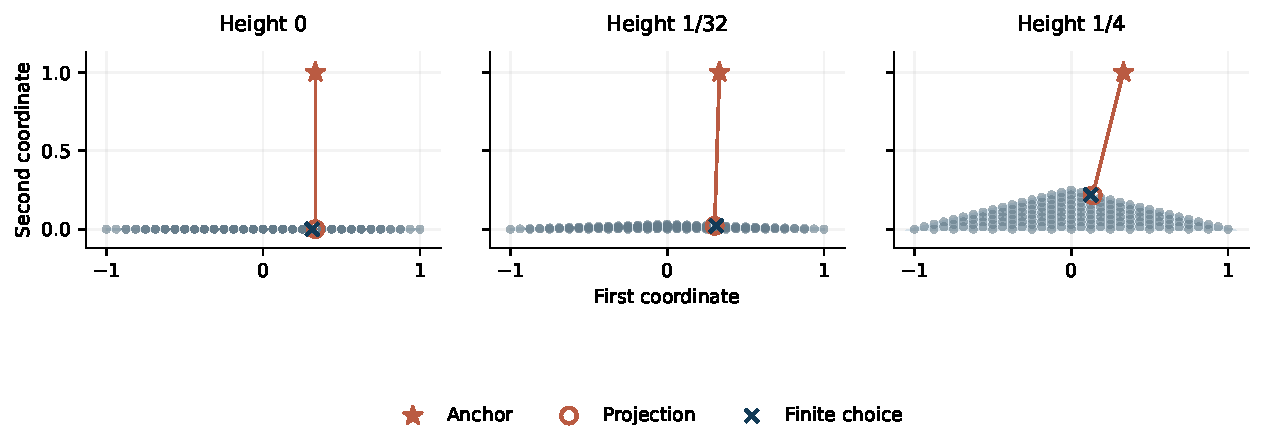
\includegraphics[width=\textwidth]{figures/convex_projection.pdf}
\caption{The same finite-cloud construction for a segment and two thin triangles, with anchor $(1/3,1)$. Gray points use rational simplex weights of denominator sixteen. The finite choice approaches the unique Euclidean projection without testing affine rank. Exact fractions determine the selected points; floating-point coordinates are used only for this illustration.}
\end{figure}

\subsection{Two boundaries that the theorem does not remove}

\paragraph{Hausdorff coherence alone does not stabilize nearest points.}
For \(n\geq1\), let
\[
 S_n=\{-1,\,1+(-1)^n2^{-n}\}\subset\mathbb Q,
 \qquad z=0.
\]
The clouds satisfy \(H_\infty(S_n,S_m)\leq r_n+r_m\).
Their exact nearest point is uniquely \(-1\) for even \(n\), and
uniquely \(1-2^{-n}\) for odd \(n\).  Thus the independently selected
minimizers do not form a Cauchy sequence.  This example involves no tie
ambiguity.  The missing hypothesis is asymptotic midpoint closure: the
limit cloud is the nonconvex set \(\{-1,1\}\).

\paragraph{An equation does not automatically provide a Hausdorff name.}
For a real coefficient \(a\), consider the nonempty compact convex set
\[
 K_a=\{x\in[-1,1]: ax=0\}.
\]
If \(a=0\), then \(P_{K_a}(1)=1\); if \(a\ne0\), then
\(P_{K_a}(1)=0\).  The set-valued input jumps at zero, and so does this
projection.  A finite-observation algorithm cannot produce this projection
uniformly from an arbitrary Cauchy name of \(a\): an observation consistent
with zero is also consistent with a sufficiently small nonzero rational.
Convexity does not remove the need to supply or derive a Hausdorff
presentation of the solution set.  For exact rational \(a\), equality is
decidable and this particular obstruction disappears; the two input
representations must not be conflated.

\subsection{Arithmetic proof audit and Lean completion obligations}

Every executable step uses finite lists, positive-denominator rational
arithmetic, bounded minima, bounded maxima, coordinate sums, or an explicit
dyadic schedule.  Dimension and vertex count may be numerical inputs.
To express the construction in the repository's object theory, encode a
rational as a signed numerator and positive natural denominator; encode a
point and a cloud by the existing sequence programs.  Comparisons are
cross-multiplied integer inequalities.  The guard that denominators are
positive is retained at every division and floor operation.

The essential induction invariants are as follows.
\begin{enumerate}
\item During a finite minimum scan, the saved index is below the processed
      prefix length and its squared-distance score is at most every score
      in that prefix.  The bounded universal comparison is represented by
      the existing Boolean-fold predicate.
\item During a coordinate sum, the partial difference of the two squared
      distances is bounded by \(4B\) times the processed coordinate count
      times the prescribed maximum-norm error.
\item During simplex rounding, the partial sum of floor values is at most
      \(D\), and the accumulated weight error is below the processed
      count divided by \(D\).  The last coordinate is explicitly the
      remaining weight.
\item During enumeration of weight codes, the retained list contains
      exactly the processed tuples with nonnegative entries and sum \(D\).
\end{enumerate}
Each invariant becomes a quantifier-free equation or inequality after
Booleanizing bounded comparisons.  Arbitrarily large numerical loops do
not introduce stronger induction.  Conversely, an abstract Lean proof
using real compactness is not a substitute for these arithmetic
derivations.

The complete Lean path is concrete:
\begin{enumerate}
\item Reuse finite least-argmin, rational arrays, Hausdorff witnesses, and
      bounded reflection from the existing \texttt{Derivations} project.
      Define \texttt{sqDist}, \texttt{cloudMidpointDefect}, and the
      rational \texttt{pick} program.
\item Prove the coordinate polynomial identity and the Lipschitz estimate
      in object arithmetic.  Export the finite comparison theorem as
      a theorem of the form \texttt{Gamma |- [PRAAx] cloudPairBound},
      keeping the cloud hypotheses inside the object formula.
\item Compose that theorem with the existing dyadic-order and
      regular-name modules to prove \eqref{eq:cloud-name}.  The essential
      proof term consumes pairwise finite contracts and performs no
      induction on the unbounded statement ``all later stages are close.''
\item Implement and prove the simplex rounding producer, then specialize
      the generic cloud theorem to \eqref{eq:hull-cloud}.  Bounded
      enumeration has the explicit cap \((D_n+1)^m\).
\item Export represented membership and the minimum-property comparison
      using finite covers and rational slack removal.  Finally prove an
      ordinary Lean semantic interpretation identifying the represented
      point with Euclidean projection.
\end{enumerate}
The present section supplies full human proofs of the finite estimates and
the producer.  The object-language and semantic Lean endpoints are
formalization targets unless a separate build record explicitly marks
them checked.  The included exact-rational program exercises the actual
rounding, finite minimization, and cross-cloud inequality; those executions
validate the implementation examples, not the universal theorem.
